\subsection{Praktična primjena matematičkog modela}\label{sec:prakticna}
Definiranjem matematičkog modela prigušenog sustava s jednim stupnjem slobode,
pobuđenog sinusnom silom postavljeni su temelji za eksperimentalno određivanje
stupnja prigušenja i prirodne frekvencije. Stupnanj prigušenja jest veličina od
izuzetne praktične važnosti, a nije ga moguće odrediti teoretski iz projektnih
parametara, već se mora odrediti eksperimentalno (~\cite{dk_skripta}). %Isto tako izmjerena vrijednost prirodne
%frekvencije jest stvarno svojstvo konstrukcije, s kojim se uspoređuje teoretski
%određena prirodna frekvencija. 
Ispitivanje koje će biti razmatrano u ovome radu naziva se \textit{rezonancijski
pokus}.

%Matematički model prigušenog sustava s jednim stupnjem slobode, pobuđen sinusnom
%silom koristi se priklikom određivanja stupnja prigušenja i prirodne frekvencije 
%realnih konstrukcija. Stupanj prigušenja je veličina od izuzetne važnosti koju nije
%moguće odrediti analitički, nego ju je potrebno odrediti ispitivanjima. 

Ispitivanja se provode \textit{vibracijskim uređajem}. Vibracijski uređaj se sastoji
od dvije košare sa utezima na uspravnoj osovini koje rotiraju u suprotnim smjerovima
konstantnom kutnom brzinom $\omega$. Osovina je pričvršćena za metalnu ploču koja se
kruto povezuje s građevinom (~\cite{dk_skripta}). 

\begin{figure}[H]
        \begin{subfigure}[b][][l]{0.45\textwidth}
        \input{./skice/sdf/vibracijski-t0}
        \caption{}
        \label{fig:vibracijski-t0}
    \end{subfigure}
    \hfill
    \begin{subfigure}[b][][r]{0.45\textwidth}
        \input{./skice/sdf/vibracijski-t}
        \caption{}
        \label{fig:vibracijski-t}
    \end{subfigure}
    \caption{Shematski prikaz vibracijskog uređaja: 
            (\subref{fig:vibracijski-t0}) u inicijalnom položaju;
            (\subref{fig:vibracijski-t}) položaj nakon vremena t}
    \label{fig:vibracijski}
\end{figure}

Sila pobude građevine jest ukupna centrifugalna sila vibracijskog uređaja, koja je 
jednaka je sumi centrifugalnih sila pojedinih masa.
Horizontalne komponente su jednakog intenziteta ali suprotnog smjera pa se
poništavaju, stoga sila pobude je jednaka sumi vertikalnih komponenti, odnosno:
\begin{equation}
    p(t)=(m_ee\omega^2)\sin(\omega t)
\end{equation}

Odziv sustava s jednim stupnjem slobode na pobudu vibracijskim uređajem opisan je
slijedećom diferencijalnom jednadžbom:
\begin{equation}
    m\ddot{u}+c\dot{u}+ku=(m_ee\omega^2)\sin(\omega t)
\end{equation}

Amplituda prisilnog pomaka glasi (iz \eqref{eq:prisilni_alternativno_rjesenje_Rd}):
\begin{equation}
    u_0=\frac{m_ee}{k}\omega^2R_d = \frac{m_ee}{m}\left(\frac{\omega}{\omega_n}\right)^2R_d
\end{equation}

Amplituda prisilnog ubrzanja (iz \eqref{eq:R_a}):
\begin{equation}
    \ddot{u}_0=\frac{m_ee}{m}\omega^2R_a=\frac{m_ee\omega_n^2}{m}\left(\frac{\omega}{\omega_n}\right)^2R_a
\end{equation}

\begin{figure}[H]
    \input{./grafovi/sdf/ra-vibracijski}
    \caption{Amplituda ubrzanja u ovisnosti o omjeru frekvencija}
    \label{fig:ra-vibracijski}
\end{figure}

Na grafu sa slike \ref{fig:ra-vibracijski} vidljivo je da daljnjim porastom frekvencije pobude (iznad prirodne
frekvencije) amplituda prisilnog ubrzanja raste. Navedeni rast se događa jer je
amplituda pobude proporcionalna s $\omega^2$. 
\par

Za određivanje stupnja prigušenja i prirodne frekvencije vrši se
\textit{rezonancijski pokus}, a temelji se na slijedećoj relaciji (iz \eqref{eq:frf_rezonanca})
\begin{equation}\label{eq:rezonancijski_pokus}
    \zeta = \frac{1}{2}\frac{(u_{st})_0}{(u_0)_{\omega=\omega_n}}
\end{equation}
Potrebno je eksperimentalno odrediti amplitudu statičkog pomaka i prirodnu frekvenciju. 
%U eksperimentima se redovito mjeri amplituda ubrzanja a amplitudu pomaka možemo
%dobiti slijedećom relacijom:
%\begin{equation}
%    u_0=\frac{\ddot{u}_0}{\omega^2}
%\end{equation}

Prirodna frekvencija se određuje na slijedeći način:
\begin{enumerate}
    \item pobuđivanje konstrukcije vibracijskim uređajem namještenim na
        određenu frekvenciju $\omega$.
    \item očitavanje faznog kuta. Ako je fazni kut $\phi = 90\degree$, tada je
        prirodna frekvencija $\omega_n$ jednaka frekvenciji pobude $\omega$.
    \item nakon što isčezne prolazni dio odziva, očitava se amplituda prisilnog ubrzanja
\end{enumerate}

Amplitudu prisilnog pomaka možemo dobiti iz amplitude prisilnog ubrzanja korištenjem
slijedeće formule (iz (~\cite{dk_skripta})):
\begin{equation}
    u_0=\frac{(\ddot{u}_0)_{\omega=\omega_n}}{(\omega^2)_{\omega=\omega_n}} \quad
    \text{ jer je } \quad
    \ddot{u}(t) = -u_0\omega^2\sin(\omega t -\phi), \quad
\end{equation}

Da bi bilo moguće odrediti prigušenje sustava prema formuli \eqref{eq:rezonancijski_pokus} 
potrebno je odrediti amplitudu statičkog pomaka $(u_{st})_0=p_{0,max}/k$, gdje je
$p_{0,max}$ amplituda pobude u rezonanci. Amplituda statičkog pomaka se
\textbf{mora} odrediti pokusom, a ne izračunati prema relaciji $p_0/k$ zato što $k$
nije eksperimentalno određen.Vibracijskim uređajem je vrlo teško (ili
nemoguće) prouzročiti veliku \textbf{statičku} silu pobude. Dva su pristupa rješavanju
navedenog problema:
\begin{enumerate}
    \item Sporim rotiranjem velikih masa - Nije najbolje rješenje jer je sila pobude
        proporcionalna s kvadratom kutne brzine rotacije utega. Stoga i za velike mase 
        utega amplituda sile pobude je relativno mala.
    \item Povlačenjem konstrukcije užetom silom koja je jednaka amplitudi sile
        pobude vibracijskim uređajem $p_{0,max}$.
\end{enumerate}

Osim rezonancijskim pokusom, prigušenje i prirodnu frekvenciju moguće je
odrediti \textbf{frekvencijskim krivuljama odziva}. Postupak je slijedeći:
\begin{enumerate}
    \item pobuđivanje konstrukcije vibracijskim uređajem namještenim na određenu
        frekvenciju
    \item određivanje amplitude \textbf{prisilnog} dijela 
    \item namještanje vibracijskog uređaja na drugu frekvenciju, te ponavljanje
        postupka%\footnote{Frekvencije vibracijskog uređaja nalaze se u širem spektru 
%        frekvencija, koji uključuje rezonantnu frekvenciju i frekvencije iz njezine 
%        okoline (i lijevo i desno).} 
\end{enumerate}

Frekvencijska krivulja odziva iscrtava se iz izmjerenih podataka. Frekvencijske
funkcije odziva mogu prikazivati slijedeće ovisnosti:
\begin{enumerate}
    \item ovisnost amplituda ubrzanja o frekvencijskom omjeru - izravno iz
        izmjerenih podataka. Bitno je za naglasiti da je navedena krivulja
        proporcionalna s $\omega^2$.

    \item ovisnost dinamičkog faktora ubrzanja o frekvencijskom omjeru (konstantna
        amplituda pobude) - dijeljenjem izmjerenih podataka s $\omega^2$ 

    \item ovisnost dinamičkog faktora pomaka o frekvencijskom omjeru (konstantna
        amplituda pobude) - dijeljenjem izmjerenih podataka s $\omega^4$.
\end{enumerate}

Stupanj prigušenja i prirodna frekvencija može se odrediti iz bilo koje od navedenih
krivulja. Prirodna frekvencija jednaka je frekvenciji sile pobude u rezonanci.
Stupanj prigušenja određuje se iz \textit{pojasa polovice snage} jednadžbom
\eqref{eq:hpb_zeta_f}, što znači da je potrebno odrediti amplitudu odziva pri
rezonanci te frekvencije za koje je amplituda odziva jednaka $r_{res}/\sqrt{2}$.
\begin{figure}[H]
    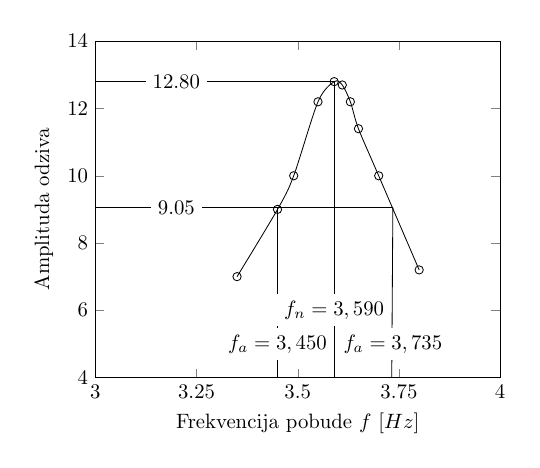
\begin{tikzpicture}[scale=0.75]
    \begin{axis} [
        ylabel = Amplituda odziva,
        xlabel = {Frekvencija pobude $f$ $[Hz]$},
        xmin = 3, xmax = 4,
        ymin = 4, ymax = 14,
        xtick = {3.0, 3.25, 3.5, 3.75, 4.0},
%        grid=both,
     ]
        \draw (3.35, 7)  circle[radius=2pt,fill=none,color=black]; 
        \draw (3.45, 9) circle[radius=2pt,fill=none,color=black];
        \draw (3.49, 10) circle[radius=2pt,fill=none,color=black];
        \draw (3.55,12.2) circle[radius=2pt,fill=none,color=black];
        \draw (3.59,12.8) circle[radius=2pt,fill=none,color=black];
        \draw (3.61,12.7) circle[radius=2pt,fill=none,color=black];
        \draw (3.63,12.2) circle[radius=2pt,fill=none,color=black];
        \draw (3.65,11.4) circle[radius=2pt,fill=none,color=black];
        \draw (3.7,10) circle[radius=2pt,fill=none,color=black];
        \draw (3.8,7.2) circle[radius=2pt,fill=none,color=black];
        
        \draw plot [smooth] coordinates{
            (3.35, 7)
            (3.45, 9) 
            (3.49, 10) 
            (3.55,12.2) 
            (3.59,12.8) 
            (3.61,12.7) 
            (3.63,12.2) 
            (3.65,11.4) 
            (3.7,10) 
            (3.8,7.2) 
        };

        %amplituda rezonance
        \draw[thin] (0, 12.8) -- (3.59, 12.8);
        \draw[thin] (3.59, 0) -- (3.59, 12.8);

        %amplituda pojasa polovice snage
        \draw[thin] (0, 9.05) -- (3.735,9.05);
        \draw[thin] (3.45, 0) -- (3.45, 9.05);
        \draw[thin] (3.73, 0) -- (3.735,9.05);

        %oznake frekvencija
        \node[rectangle,fill=white] at (3.59,6) {$f_n=3,590$};
        \node[rectangle,fill=white] at (3.45,5) {$f_a=3,450$};
        \node[rectangle,fill=white] at (3.735,5) {$f_a=3,735$};

        %oznake amplituda
        \node[rectangle,fill=white] at (3.2,12.8) {$12.80$};
        \node[rectangle,fill=white] at (3.2,9.05) {$9.05$};

    \end{axis}
\end{tikzpicture}

    \caption{Frekvencijska funkcija odziva konstruirana pomoću mjerenih podataka}
    \label{fig:frf-poku}
\end{figure}
